% --------------------------------------------------------------------------- %
% A0 paper poster for MetrumRG						   %
% --------------------------------------------------------------------------- %
% Created with Brian Amberg's LaTeX Poster Template. 					     %
% --------------------------------------------------------------------------- %

\documentclass[portrait,fontscale=0.46,paperwidth=36in,paperheight=48in]{baposter}

\usepackage{relsize}		% For \smaller
\usepackage{url}			% For \url
\usepackage{epstopdf}	% Included EPS files automatically converted to PDF to include with pdflatex

\usepackage[bitstream-charter]{mathdesign}
\usepackage[T1]{fontenc}

% Deprecating osfigures option; use oldstyle instead; 2020-09-10
\usepackage[defaultsans,oldstyle,scale=0.95]{opensans}

\usepackage{vwcol} 
\usepackage{multicol}
\usepackage[font=small,labelfont=bf]{caption} % Required for specifying captions to tables and figures

% Added for figures
\usepackage{float}
\usepackage{wrapfig}
\usepackage{threeparttable}


%%% Global Settings %%%%%%%%%%%%%%%%%%%%%%%%%%%%%%%%%%%%%%%%%%%%%%%%%%%%%%%%%%%

\graphicspath{{pix/}}	% Root directory of the pictures 
\tracingstats=2			% Enabled LaTeX logging with conditionals

%%% Color Definitions %%%%%%%%%%%%%%%%%%%%%%%%%%%%%%%%%%%%%%%%%%%%%%%%%%%%%%%%%

\definecolor{bordercol}{RGB}{40,40,40}
\definecolor{headercol1}{RGB}{186,215,230}
\definecolor{headercol2}{RGB}{80,80,80}
\definecolor{headerfontcol}{RGB}{0,0,0}
\definecolor{boxcolor}{RGB}{186,215,230}
\definecolor{metgreen}{rgb}{0,0.555,0}
\definecolor{lightergreen}{rgb}{.8,1,0.85}
\definecolor{lightergray}{RGB}{225,225,225}
\definecolor{darkteal}{RGB}{41, 127, 157}
\definecolor{tealdark}{RGB}{41, 104, 157}
\definecolor{black}{RGB}{0,0,0}
\definecolor{red}{RGB}{180, 55, 87}
\definecolor{Mgreen_official}{RGB}{9,101,46}

%%% Metrum's official green RGB is weirdly greyish-green so using
% the green below to get a close match to the Metrum M
\definecolor{Mgreen}{RGB}{0, 120,  50}

\newcommand{\figtxt}[1]{\textcolor{Mgreen}{\textit{#1 }}}
\newcommand{\figtxtG}[1]{\textcolor{Mgreen}{\textit{#1 }}}
\newcommand{\figtxtT}[1]{\textcolor{Mgreen}{\textbf{(#1)}}}
\newcommand{\greenBF}[1]{\textcolor{Mgreen}{\textbf{#1}}}

% PLEASE MODIFY COLOR SCHEME HERE IF NEEDED
\colorlet{titlefgcol}{black}
\colorlet{headerbgcol}{Mgreen}
\colorlet{headerfgcol}{white}
\colorlet{bordercol}{lightergray}
\newcommand{\headershade}{none}

\usepackage{tcolorbox}
\newtcolorbox{demobox}[1][]{colback=Mgreen!5!white,colframe=Mgreen!90!black,width=0.48\linewidth,nobeforeafter,box align=top,before=\noindent,#1}
\newtcolorbox{demobx}[1][]{colback=white,colframe=Mgreen,width=0.98\linewidth,nobeforeafter,box align=top,before=\noindent,#1}


\newenvironment{ColFigure}
  {\par\medskip\noindent\minipage{\linewidth}}
  {\endminipage\par\medskip}

  \usepackage[normalem]{ulem}

%%%%%%%%%%%%%%%%%%%%%%%%%%%%%%%%%%%%%%%%%%%%%%%%%%%%%%%%%%%%%%%%%%%%%%%%%%%%%%%%
%%% Utility functions %%%%%%%%%%%%%%%%%%%%%%%%%%%%%%%%%%%%%%%%%%%%%%%%%%%%%%%%%%

%%% Save space in lists. Use this after the opening of the list %%%%%%%%%%%%%%%%
\newcommand{\compresslist}{
	\setlength{\itemsep}{1pt}
	\setlength{\parskip}{0pt}
	\setlength{\parsep}{0pt}
}

%%%%%%%%%%%%%%%%%%%%%%%%%%%%%%%%%%%%%%%%%%%%%%%%%%%%%%%%%%%%%%%%%%%%%%%%%%%%%%%
%%% Document Start %%%%%%%%%%%%%%%%%%%%%%%%%%%%%%%%%%%%%%%%%%%%%%%%%%%%%%%%%%%%
%%%%%%%%%%%%%%%%%%%%%%%%%%%%%%%%%%%%%%%%%%%%%%%%%%%%%%%%%%%%%%%%%%%%%%%%%%%%%%%

\begin{document}
\typeout{Poster rendering started}

%%% Setting Background Image %%%%%%%%%%%%%%%%%%%%%%%%%%%%%%%%%%%%%%%%%%%%%%%%%%
\background{
%	\begin{tikzpicture}[remember picture,overlay]%
%	\draw (current page.north west)+(-2em,2em) node[anchor=north west]
%	{\includegraphics[height=1.1\textheight]{background}};
%	\end{tikzpicture}
}

%%% General Poster Settings %%%%%%%%%%%%%%%%%%%%%%%%%%%%%%%%%%%%%%%%%%%%%%%%%%%
%%%%%% Eye Catcher, Title, Authors and University Images %%%%%%%%%%%%%%%%%%%%%%
\begin{poster}{
	grid=false,
	% Option is left on true though the eyecatcher is not used. The reason is
	% that we have a bit nicer looking title and author formatting in the headercol
	% this way
	% columns = 4,
	eyecatcher=false, 
	borderColor=bordercol,
	headerColorOne=headerbgcol,
	headerColorTwo=headerbgcol,
	headerFontColor=headerfgcol,
	% Only simple background color used, no shading, so boxColorTwo isn't necessary
	boxColorOne=white,
	headershape=rectangle,
	headerfont=\Large\bf\textsf,
	textborder=rectangle,
	background=user,
	headerborder=open,
  boxshade=none, 
  headershade=plain,
  headerheight=0.1\textheight %% CHANGE THIS TO INCREASE ROOM FOR LONG TITLE
}
%%% Eye Cacther %%%%%%%%%%%%%%%%%%%%%%%%%%%%%%%%%%%%%%%%%%%%%%%%%%%%%%%%%%%%%%%
{
%	Eye Catcher, empty if option eyecatcher=false - unused
}
%%% Title %%%%%%%%%%%%%%%%%%%%%%%%%%%%%%%%%%%%%%%%%%%%%%%%%%%%%%%%%%%%%%%%%%%%%
{
	\textbf{\textsf{\color{titlefgcol}{
	A Suite of Open-Source Tools to Guide Efficient Pharmacometric Analyses
	 }}}\vspace{.5em}
}
%%% Authors %%%%%%%%%%%%%%%%%%%%%%%%%%%%%%%%%%%%%%%%%%%%%%%%%%%%%%%%%%%%%%%%%%%
{
	Katherine Kay, Ph.D.$^\ast$$^1$, Kyle Baron, Pharm.D. Ph.D.$^\ast$$^1$, Seth Green M.S.$^1$, 
	Samuel Callisto, Ph.D.$^1$, Curtis Johnston, Pharm.D.$^1$, Kyle Barrett, M.S.$^1$, \\
	Devin Pastoor, Ph.D.$^1$$^,$$^2$, Jim Rogers, Ph.D.$^1$, Ana Ruiz-Garcia, Pharm.D. Ph.D.$^1$$^,$$^3$, 
	Tim Waterhouse, Ph.D.$^1$, Matthew Wiens, M.A.$^1$, Matthew Riggs, Ph.D.$^1$ \\ \\
	{\smaller$^\ast$These authors contributed equally to this work \\
	  $^1$\textit{Metrum Research Group, Tariffville, CT, USA}, $^2$\textit{Posit (formerly RStudio), Boston, MA, USA (current)}, $^3$\textit{Gilead, City, ST, USA (current)}
	}
}
%%% Logo %%%%%%%%%%%%%%%%%%%%%%%%%%%%%%%%%%%%%%%%%%%%%%%%%%%%%%%%%%%%%%%%%%%%%%
{
% The logos are compressed a bit into a simple box to make them smaller on the result
% (Wasn't able to find any bigger of them.)
%\setlength\fboxsep{5pt}
%\setlength\fboxrule{0.5pt}
%	\fbox{
		\begin{minipage}{24em}
			\begin{center}
			%\includegraphics[width=14em]{pix/sponsorlogo.jpg}  
			%\vspace*{0.5em}
			
\includegraphics[width=21em]{pix/newlogo} 
			\end{center}
		\end{minipage}
%	}
}
%%%%%%%%%%%%%%%%%%%%%%%%%%%%%%%%%%%%%%%%%%%%%%%%%%%%%%%%%%%%%%%%%%%%%%%%%%%%%%%%
%%%%%%%%%%%%%%%%%%%%%%%%%%%%%%%%%%%%%%%%%%%%%%%%%%%%%%%%%%%%%%%%%%%%%%%%%%%%%%%%

%%%%%%%%%%% Poster specific settings %%%%%%%%%%%%%%%%%%%%%%%%%%%%%%%%%%%%%%%%%%%%%%%%%%%%%%%

% italic, left-justified text
\newcommand{\desc}[1]{
	\raggedright{\textit{#1}}
}

\newenvironment{codeFont}{\fontfamily{cmtt}\selectfont}{\par}
\newenvironment{outputFont}{\fontfamily{phv}\selectfont}{\par}

% Code block
\newcommand{\code}[1]{
	\begin{codeFont}
		\colorbox{lightergray!30}{\footnotesize{#1}}
	\end{codeFont}
	\normalsize
}
% Output block
\newcommand{\out}[1]{
	\begin{outputFont}
		\normalsize{#1}
	\end{outputFont}
	\normalsize
}

% Package Text - large, bold, green
\newcommand{\pkgText}[1]{
	\normalsize
		\greenBF{#1}
	\normalsize
}

%%%%%%%%%%% ABSTRACT %%%%%%%%%%%%%%%%%%%%%%%%%%%%%%%%%%%%%%%%%%%%%%%%%%%%%%%


\headerbox{Abstract}{name=abstract,column=0,row=0,span=3}{
	\textbf{BACKGROUND}
	Quantitative scientists are tasked with building analytical models to support decisions about complex systems. Such modeling often involves an array of processes and tools that present a challenge to collaboration and ensuring quality compliance. The objective of this work was to provide the pharmacometrics community with a suite of standardized, freely available, open-source tools to efficiently conduct traceable, reproducible, and scalable pharmacometric analyses in a controlled R environment \cite{noauthor_undated-ev}.\\
	\textbf{METHODS}
	\greenBF{Metrum Research Group has developed a suite of open-source tools that 
	can be used independently, or seamlessly integrated into a larger R-based 
	ecosystem, for pharmacometric analyses}. We have compiled example code, 
	and accompanying documentation, for each of the tasks typically required in a 
	population pharmacokinetic (PK) analysis workflow to showcase the wide-ranging 
	functionality of these tools. We considered R package management, data 
	specifications, and common modeling and simulation activities such as, exploratory 
	data analysis, executing and managing NONMEM® models and output, outcomes 
	simulation, generating diagnostic plots and parameter tables, and analysis reporting. 
	While we framed this example in the context of a simple population PK analysis, these 
	packages can also be used in other types of pharmacometric analyses, e.g., 
	pharmacokinetic-pharmacodynamic (PK-PD), quantitative systems pharmacology 
	(QSP), and statistical models.\\
	All our packages were developed and are maintained through an iterative open-source 
	software development life cycle (SDLC) \cite{Baron2021-ft}. This transparent process incorporates robust planning, iterative development, validation, and release of each package.\\
	\textbf{RESULTS}
	\greenBF{A complete, reproducible pharmacometric analysis workflow is hosted in a publicly available, 
	version-controlled repository on GitHub \cite{noauthor_2022-fh}} encompassing multiple states and stages of a 
	modeling and simulation project. In addition to the scripted example, vignettes and user guides 
	provide step-by-step directions detailing how the R packages facilitate an entire modeling and 
	simulation analysis workflow. This package ecosystem includes: bbi/bbr, lastdose, Metrum Package Network (MPN) and pkgr, mrggsave, mrgsolve, pmforest, pmplots, pmtables and yspec.\\
	\textbf{CONCLUSIONS}
	Metrum Research Group developed a suite of open-source R packages to \greenBF{support traceable, reproducible, and scalable pharmacometric analyses} and now provides the pharmacometric community with an example of how to use these tools.
\vspace{.5em}
}

%%%%%%%%%%% Flow chart %%%%%%%%%%%%%%%%%%%%%%%%%%%%%%%%%%%%%%%%%%%%%%%%%%%%%%%


\headerbox{Workflow}{name=flowchart,column=0,span=3, below=abstract}{
	\begin{figure}[H]
		\centering
		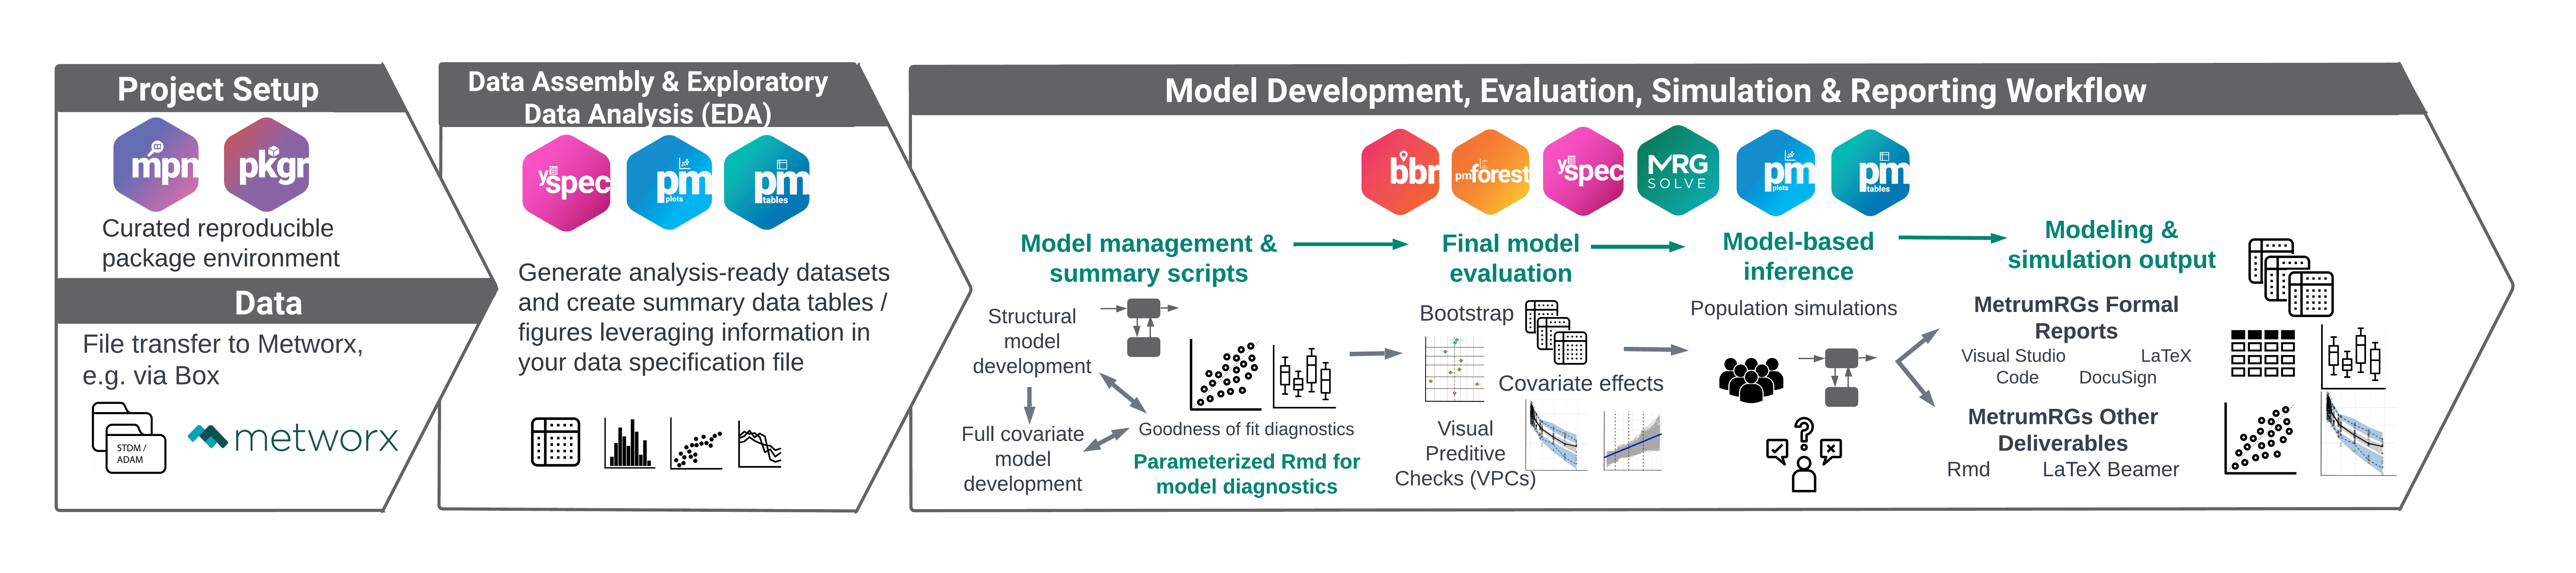
\includegraphics[scale=0.15]{"images/landscape-flowchart.png"}
	\end{figure}	
}



%%%%%%%%%%%% Large box around spot-lighted packages %%%%%%%%%%%%%%%%%%%%%%%%%%%%%%%%%%%%%%%%%%%%%%%%%%%%%%%%%

\headerbox{Package Showcase}{name=pkgs,column=0,span=3,below=flowchart}{

\noindent
% Begin the yspec box
\begin{minipage}[c]{0.333\linewidth}
	\begin{demobx}[]
	
	%%%%%%%%%%%% yspec %%%%%%%%%%%%%%%%%%%%%%%%%%%%%%%%%%%%%%%%%%%%%%%%%%%%%%%%%

	\begin{wrapfigure}{l}{0.2\textwidth}
		\vspace{-0.5cm}
		
\includegraphics[scale=0.075]{"images/ySpec-Hex.png"} 
	\end{wrapfigure}
	
	% Text chunk at the top of the box
	The \pkgText{yspec R package} is designed to help you document and manage your analysis datasets and then use this documentation throughout your project to:
	\begin{itemize}
		\vspace{-0.3cm}
		\item Guide and document the data assembly process
		\vspace{-0.2cm}
		\item Annotate figures and tables efficiently
		\vspace{-0.2cm}
		\item Manage decode values for numerically encoded discrete data items
		\vspace{-0.2cm}
		\item Make submission-ready define documents
	\end{itemize}
	\vspace{-0.2cm}

	yspec acts as a single, central location for maintaining the metadata for your analysis datasets to manage these activities.

	\vspace{1mm}
	\textbf{1. Data specifications in yaml format}

	\begin{minipage}[c]{0.55\linewidth}
		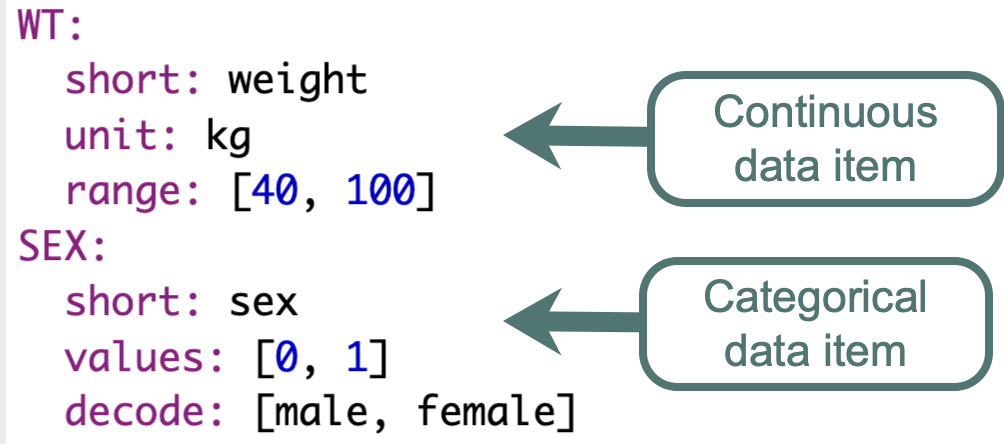
\includegraphics[scale=0.375]{"images/spec-example-2.png"} 
	\end{minipage} % no space if you need them side by side
	\begin{minipage}[c]{0.45\linewidth}
		Analysis datasets are documented in yaml format and can be loaded into R as an object. 

		\code{spec<-ys\_load("spec/analysis3.yml")\hspace{-1mm}}
	
	\end{minipage} % no space if you need them side by side
	Below we demonstrate how to use this spec object throughout all phases of project work.

	
	\vspace{1mm}
	\textbf{2. Interactive query of the analysis dataset}

	\begin{minipage}[c]{0.45\linewidth}
		\desc{Query categorical data item}
	\end{minipage} % no space if you need them side by side
	\begin{minipage}[c]{0.45\linewidth}
		% \vspace{-2mm}
		\desc{Query continuous data item}
	\end{minipage} 
	

	\begin{minipage}[c]{0.15\linewidth}
		\code{spec\$SEX}
	\end{minipage} 
	\begin{minipage}[c]{0.3\linewidth}
		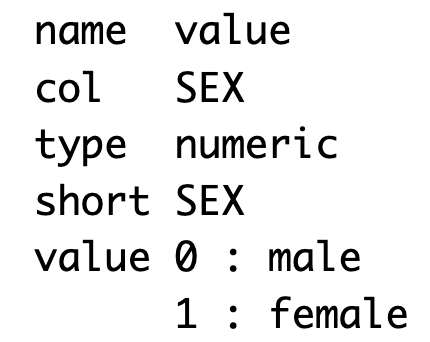
\includegraphics[scale=0.35]{"images/spec-sex.png"} 
	\end{minipage} 
	\begin{minipage}[c]{0.15\linewidth}
		\code{spec\$WT}
	\end{minipage} 
	\begin{minipage}[c]{0.25\linewidth}
		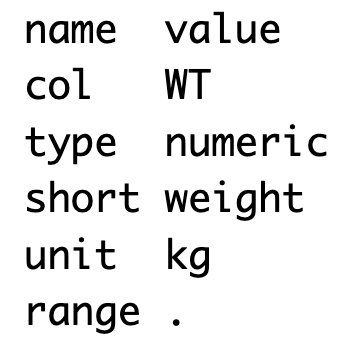
\includegraphics[scale=0.35]{"images/spec-wt.png"} 
	\end{minipage} 

	\vspace{1mm}
	\textbf{3. Validating the dataset}

	\desc{Validate the contents of your dataset against the data specification (spec) file}

	\code{ys\_check(data, spec, error\_on\_fail=FALSE)}

	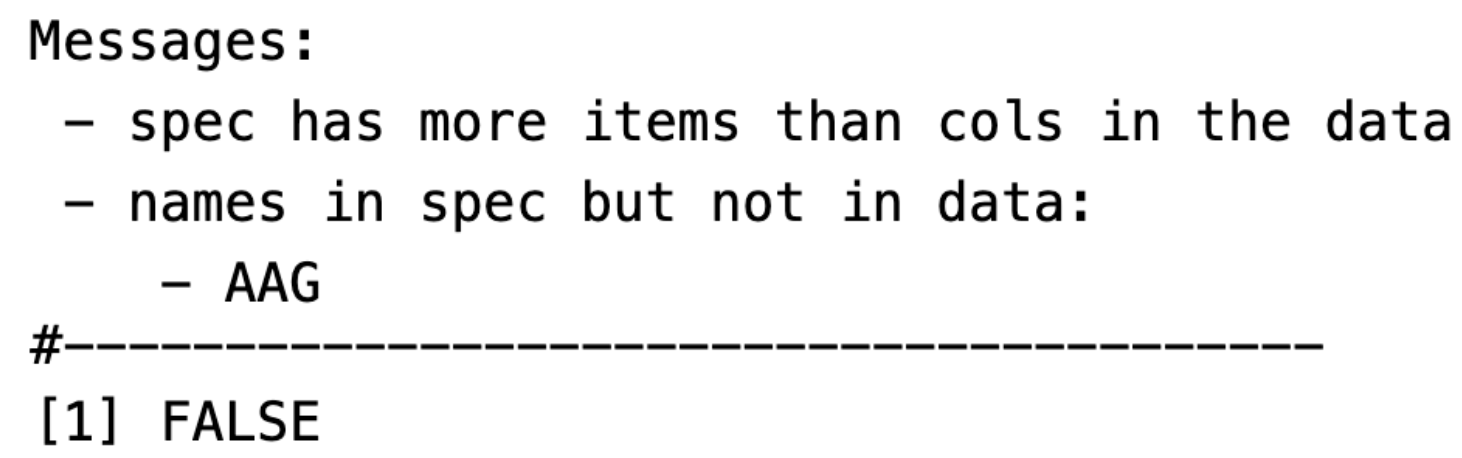
\includegraphics[scale=0.25]{"images/validate.png"} 

	\vspace{1mm}
	\textbf{4. Annotating plots and tables for project deliverables}

	\desc{Extract the short label and units for use in figure axis column labels}
	
	\code{contCovs <- axis\_col\_labs(specTex, c("AGE", "WT"), title\_case = TRUE)}

	
\includegraphics[scale=0.35]{"images/col-labs.png"} 

	\desc{Extract the short label and units for use in tables}

	\code{labs <- ys\_get\_short\_unit(specTex, parens = TRUE, title\_case=TRUE)  }
	
\includegraphics[scale=0.375]{"images/short-lab.png"} 

	\vspace{1mm}
	\textbf{5. Generate define.pdf}

	\desc{Create a define.pdf suitable for regulatory submission}

	\code{ys\_document(spec, type = "regulatory", output\_dir = "../data/derived",}

	\vspace{-0.18cm}\code{\hspace{5mm} output\_file = "define.pdf", author = "Kyle Baron")}

	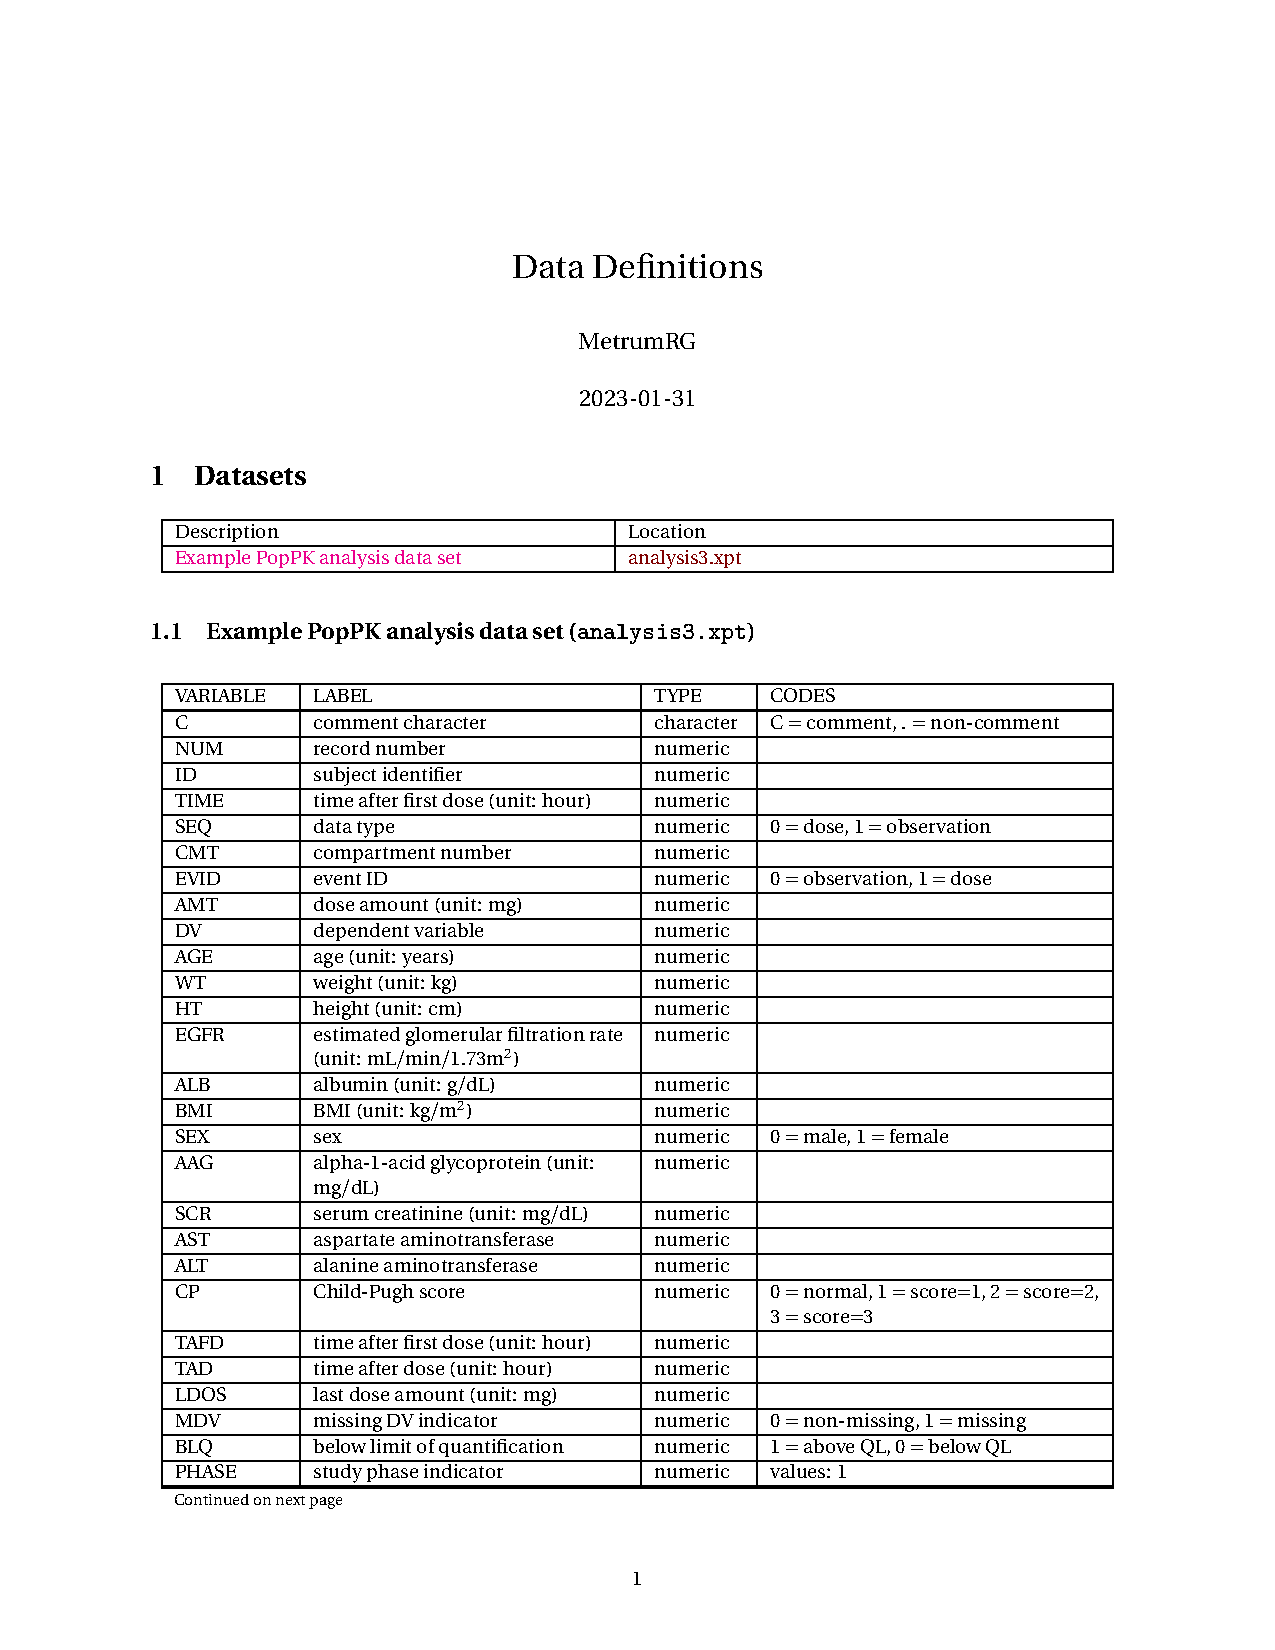
\includegraphics[scale=0.25]{"images/define.png"} 
% 	ys_document(
%   spec, 
%   type = "regulatory", 
%   output_dir = "../data/derived", 
%   output_file = "analysis2.pdf", 
%   build_dir = definetemplate(), 
%   author = "Kyle Baron"
% )

	\end{demobx}	
\end{minipage} % no space if you need them side by side
\begin{minipage}[c]{0.333\linewidth}
	\begin{demobx}[]
		% %%%%%%%%%%%% bbr %%%%%%%%%%%%%%%%%%%%%%%%%%%%%%%%%%%%%%%%%%%%%%%%%%%%%%%%%
		\begin{wrapfigure}{l}{0.2\textwidth}
			\vspace{-0.45cm}
			
\includegraphics[scale=0.15]{"images/metrum_bbr_git_logo.png"} 
		\end{wrapfigure}
		The \pkgText{bbr R package} allows you to manage, track, and report modeling activities, through simple R objects, with a user-friendly interface between R and NONMEM®. 
		bbr is used to submit models, process outputs and diagnostics, and iterate on models. It provides simple tagging and model inheritance trees to support replication and external review of your work.
		
		\textbf{1. Creating and submitting a model}

		\desc{Create your first model object from a NONMEM control stream}

		\code{mod100 <- new\_model(file.path(model\_dir, 100))}

		\desc{Submit the NONMEM model to run} 

		\code{submit\_model(mod100)}

		\vspace{1mm}
		\textbf{2. Iterative model development}

		\desc{Create a new model based on an existing model}

		\code{mod101 <- copy\_model\_from(.parent\_mod = mod100, 
			.new\_model = 101)}

		\desc{Compare a model ctl file to its parent model} \hspace{-0.75cm}

		\code{model\_diff(mod101)}

		\vspace{1mm}
		\textbf{3. Model evaluation and diagnostics}

		\begin{minipage}[c]{0.5\linewidth}
			\vspace{-2mm}
			\desc{Parse NONMEM outputs into an R list object and use it for a quick look at the model specifics, and to check if any heuristic problems were detected}

			\vspace{5mm}
			\code{sum100 <- model\_summary(mod100)}

		\end{minipage}
		\begin{minipage}[c]{0.45\linewidth}
			\vspace{-1.2mm}
			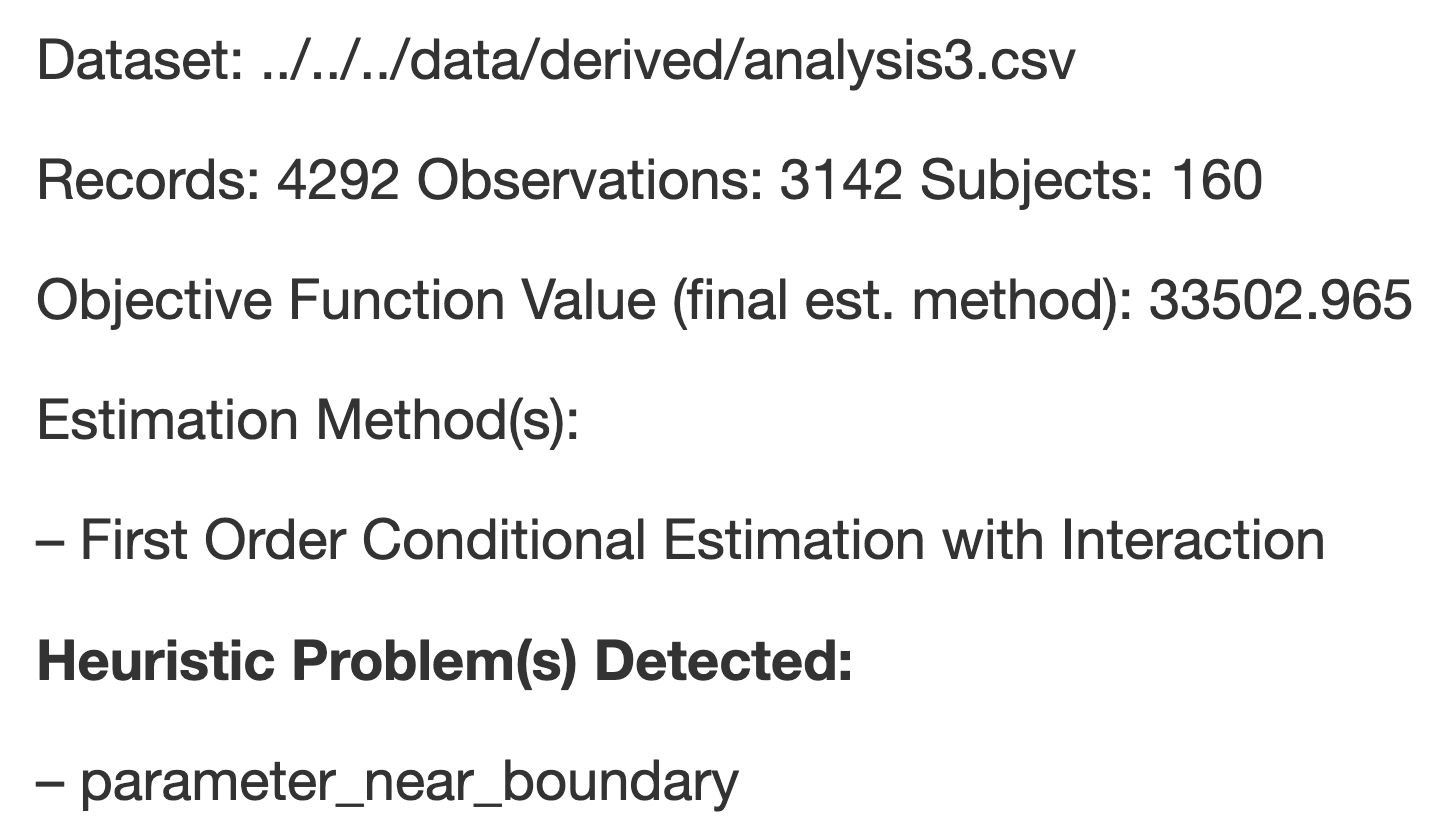
\includegraphics[scale=0.25]{"images/summary.png"} 

		\end{minipage}

		\desc{Create a simple tibble with parameter estimates}

		\code{sum100 \%>\% param\_estimates()}

		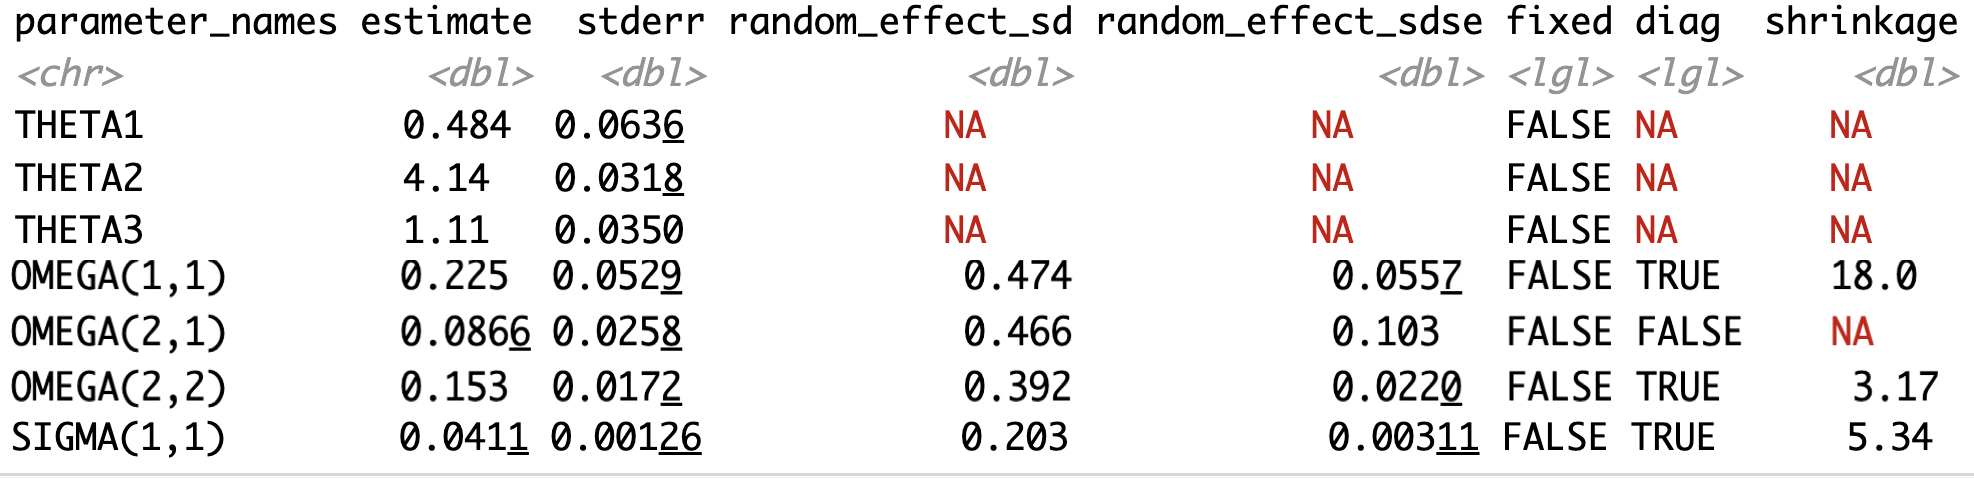
\includegraphics[scale=0.3]{"images/param-estimates-reduced.png"} 

		\begin{minipage}[c]{0.55\linewidth}
			% \desc{Generate a single data frame with model output and input data via a unique row-identifier column}

			\desc{Combine the model output and input data, via a unique row-identifier column, to create a single combined data frame}

			\code{data <- nm\_join(mod100)}

		\end{minipage}
		\begin{minipage}[c]{0.4\linewidth}
			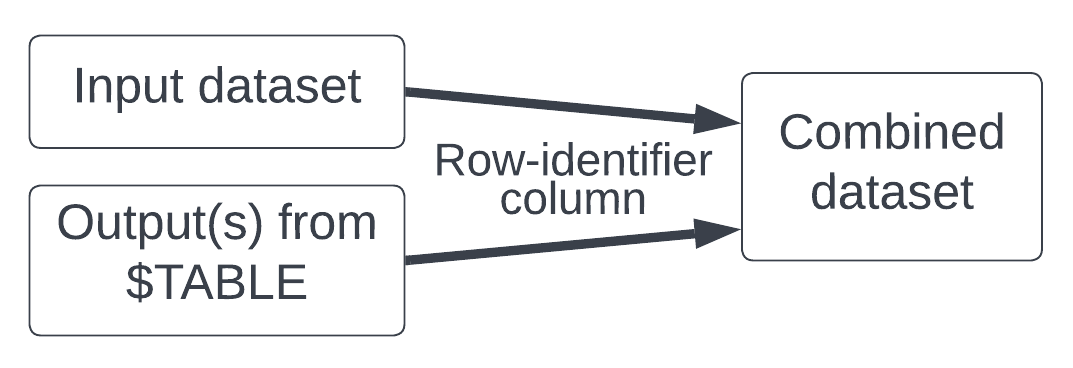
\includegraphics[scale=0.15]{"images/nm_join.png"}
		\end{minipage}
		

		The yspec package (top left) can be used to decode the categorical covariates in your data.
		
		\begin{minipage}[c]{0.6\linewidth}
			\code{data <- yspec\_add\_factors(data, spec)}
		\end{minipage}
		\begin{minipage}[c]{0.35\linewidth}
			\vspace{-4mm}
			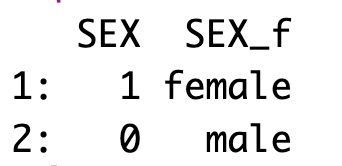
\includegraphics[scale=0.35]{"images/decode.png"} 
		\end{minipage}
		The pmplots box (top right) demonstrates how to make goodness of fit plots.

		\vspace{1mm}
		\textbf{4. Model annotation}
		
		\desc{Add notes to your model}

		\code{mod100 <- add\_notes(mod100, "systematic bias, explore alternate structure")}
		
		% \desc{Add tags to your model}
		% \code{mod100 <- mod100 \%>\% \hspace{8.7cm}}\vspace{-0.18cm}
		% \code{\hspace{0.5cm} add\_tags(c(TAGS\$one\_compartment\_absorption, TAGS\$eta\_cl, \hspace{2.25cm}}\vspace{-0.18cm}
		% \code{\hspace{2.5cm}	TAGS\$eta\_ka,	TAGS\$eta\_v,	TAGS\$proportional\_ruv)) \hspace{1.5cm}}

		\desc{Create highly customizable run logs to summarize model development}
		\code{run\_log(here("model/pk"), .recurse = FALSE) \%>\% add\_summary() \%>\%}\vspace{-0.18cm}
		\code{\hspace{0.5cm} select(run, based\_on, ofv, param\_count, notes) \hspace{2.25cm}}
		\vspace{-1mm}
		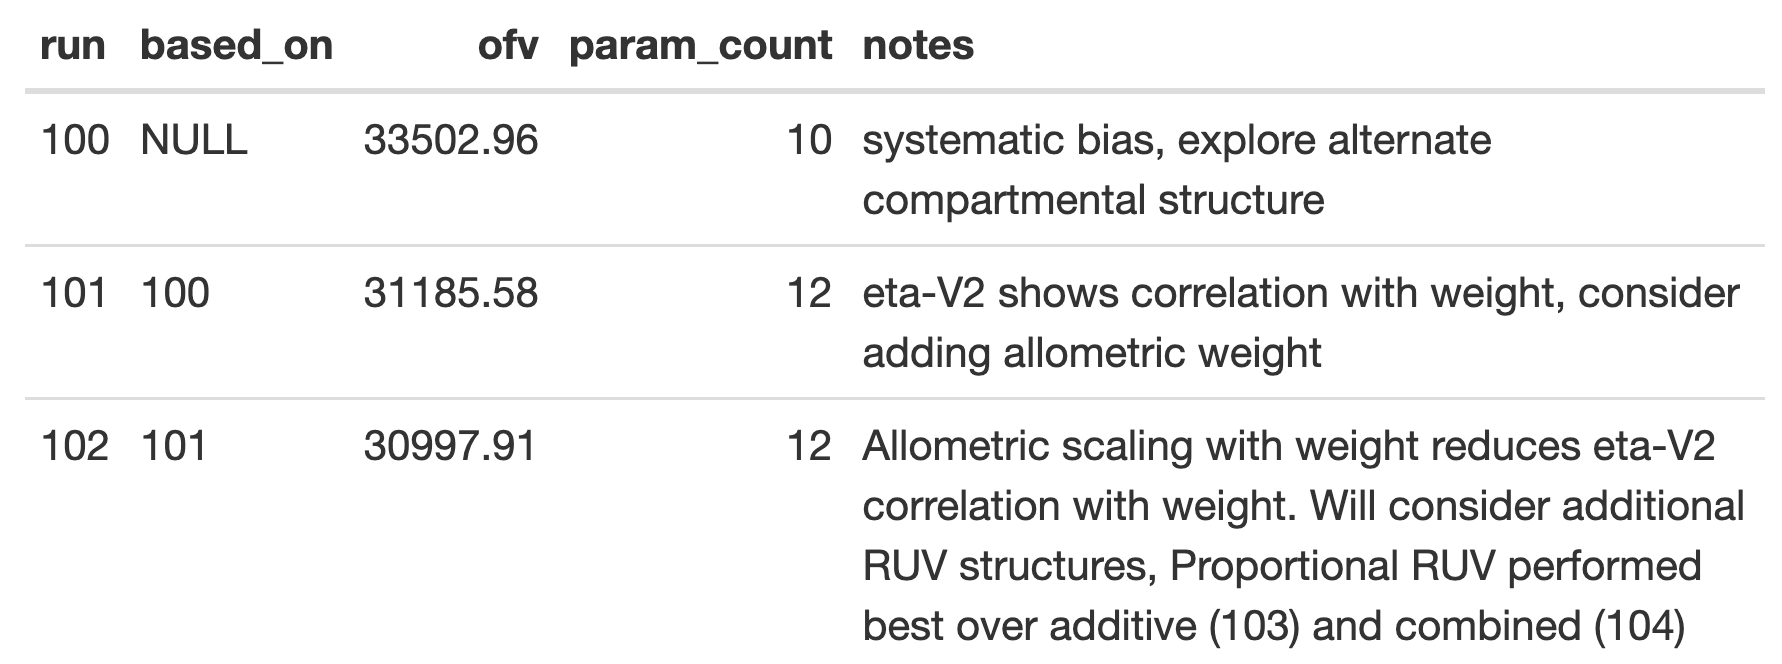
\includegraphics[scale=0.3]{"images/run-log.png"} 
		\vspace{-2mm}


	\end{demobx}	
\end{minipage} % no space if you need them side by side
\begin{minipage}[c]{0.333\linewidth}
	\vspace{-14.25cm} %%%% TODO - fix box heights

	\begin{demobx}[]

		% %%%%%%%%%%%% pmplots %%%%%%%%%%%%%%%%%%%%%%%%%%%%%%%%%%%%%%%%%%%%%%%%%%%%%%%%%

		\begin{wrapfigure}{l}{0.2\textwidth}
			\vspace{-0.45cm}
			
\includegraphics[scale=0.15]{"images/metrum_pmplots_git_logo.png"} 
		\end{wrapfigure}
		% Text chunk at the top of the box
		The \pkgText{pmplots R package} allows you to make simple, standardized plots in a pharmacometric data analysis environment. The package provides a standard set of commonly used plots in pharmacometric analyses, as opposed to generating a new grammar of graphics.


		%%% DV - PRED section
		
		\begin{minipage}[t]{0.6\textwidth} %% Code
			\vspace{-9mm}
			% DV-PRED
			\desc{Observed versus population predictions}
			\code{p1 <- dv\_pred(data)}
			%DV-IPRED
			\desc{Observed versus individual predictions}
			\code{p2 <- dv\_ipred(data)}
		% Combine
			\desc{Combine for output:}\hspace{-0.75cm} \code{p1 + p2}
		\end{minipage}	
		\begin{minipage}[c]{0.5\textwidth} %% Figure
			% \vspace{1mm}
			\hspace{-12mm}
			%DV-PRED figure
			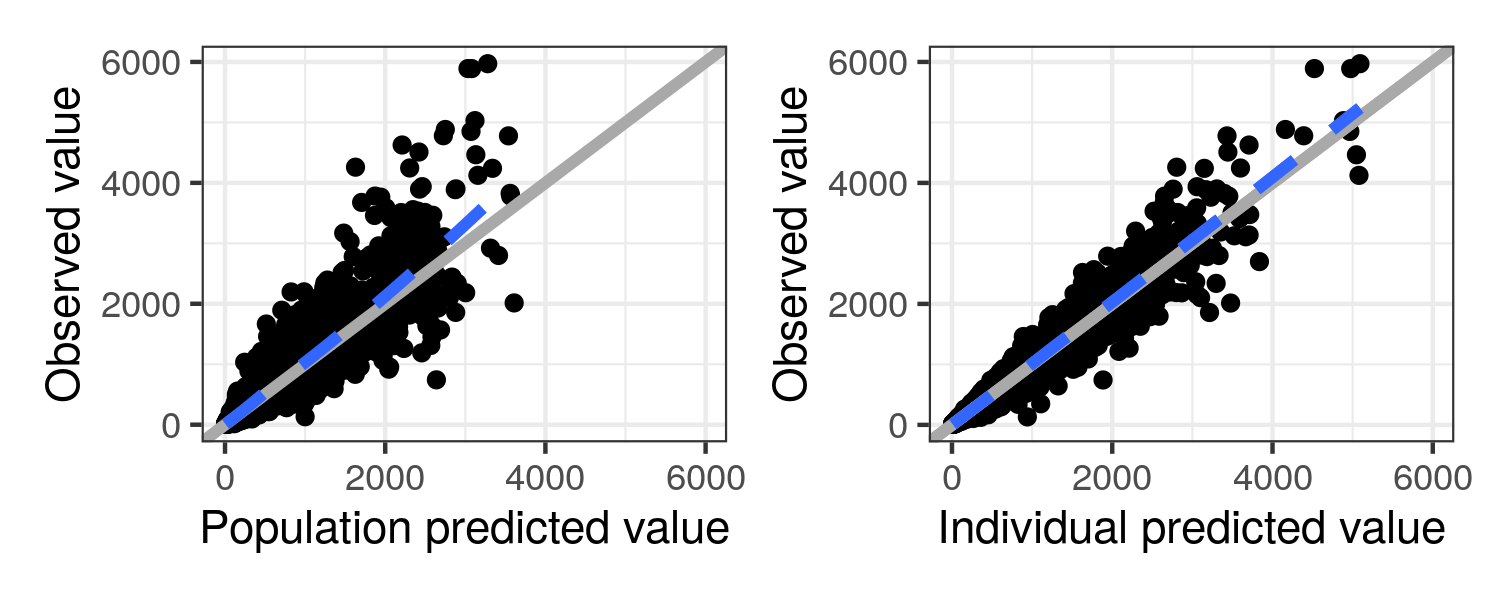
\includegraphics[scale=0.5]{"images/dv-pred-ipred.png"}
		\end{minipage}

		%%% Residuals section
		\begin{minipage}[c]{0.55\textwidth}
			\vspace{-8mm}
			 %% Code
			% CWRES - TIME
			\desc{Conditional weighted residuals versus time}\newline
			\code{p3 <- cwres\_time(data)}
			% RES - PRED
			\desc{Residuals versus population predictions}\newline
			\code{p4 <- res\_pred(data)	}
			% NPDE - Study
			\desc{NPDEs versus categorical covariate}\newline
			\code{p5 <- npde\_cat(data, \hspace{2cm} } \vspace{-0.18cm}
			\code{\hspace{2cm} x = "STUDYc//Study") }
			% WRES hist
			\desc{Histogram of weighted residuals}\newline
			\code{p6 <- wres\_hist(data)}
			% Combine
			\desc{Combine for output}
			
			% \hspace{-0.75cm} 
			\code{(p3 + p4) / (p5 + p6)}	
		\end{minipage}	
		\begin{minipage}[c]{0.5\textwidth} 
			\vspace{-6mm}
			\hspace{-6mm}
			%Residual figure
			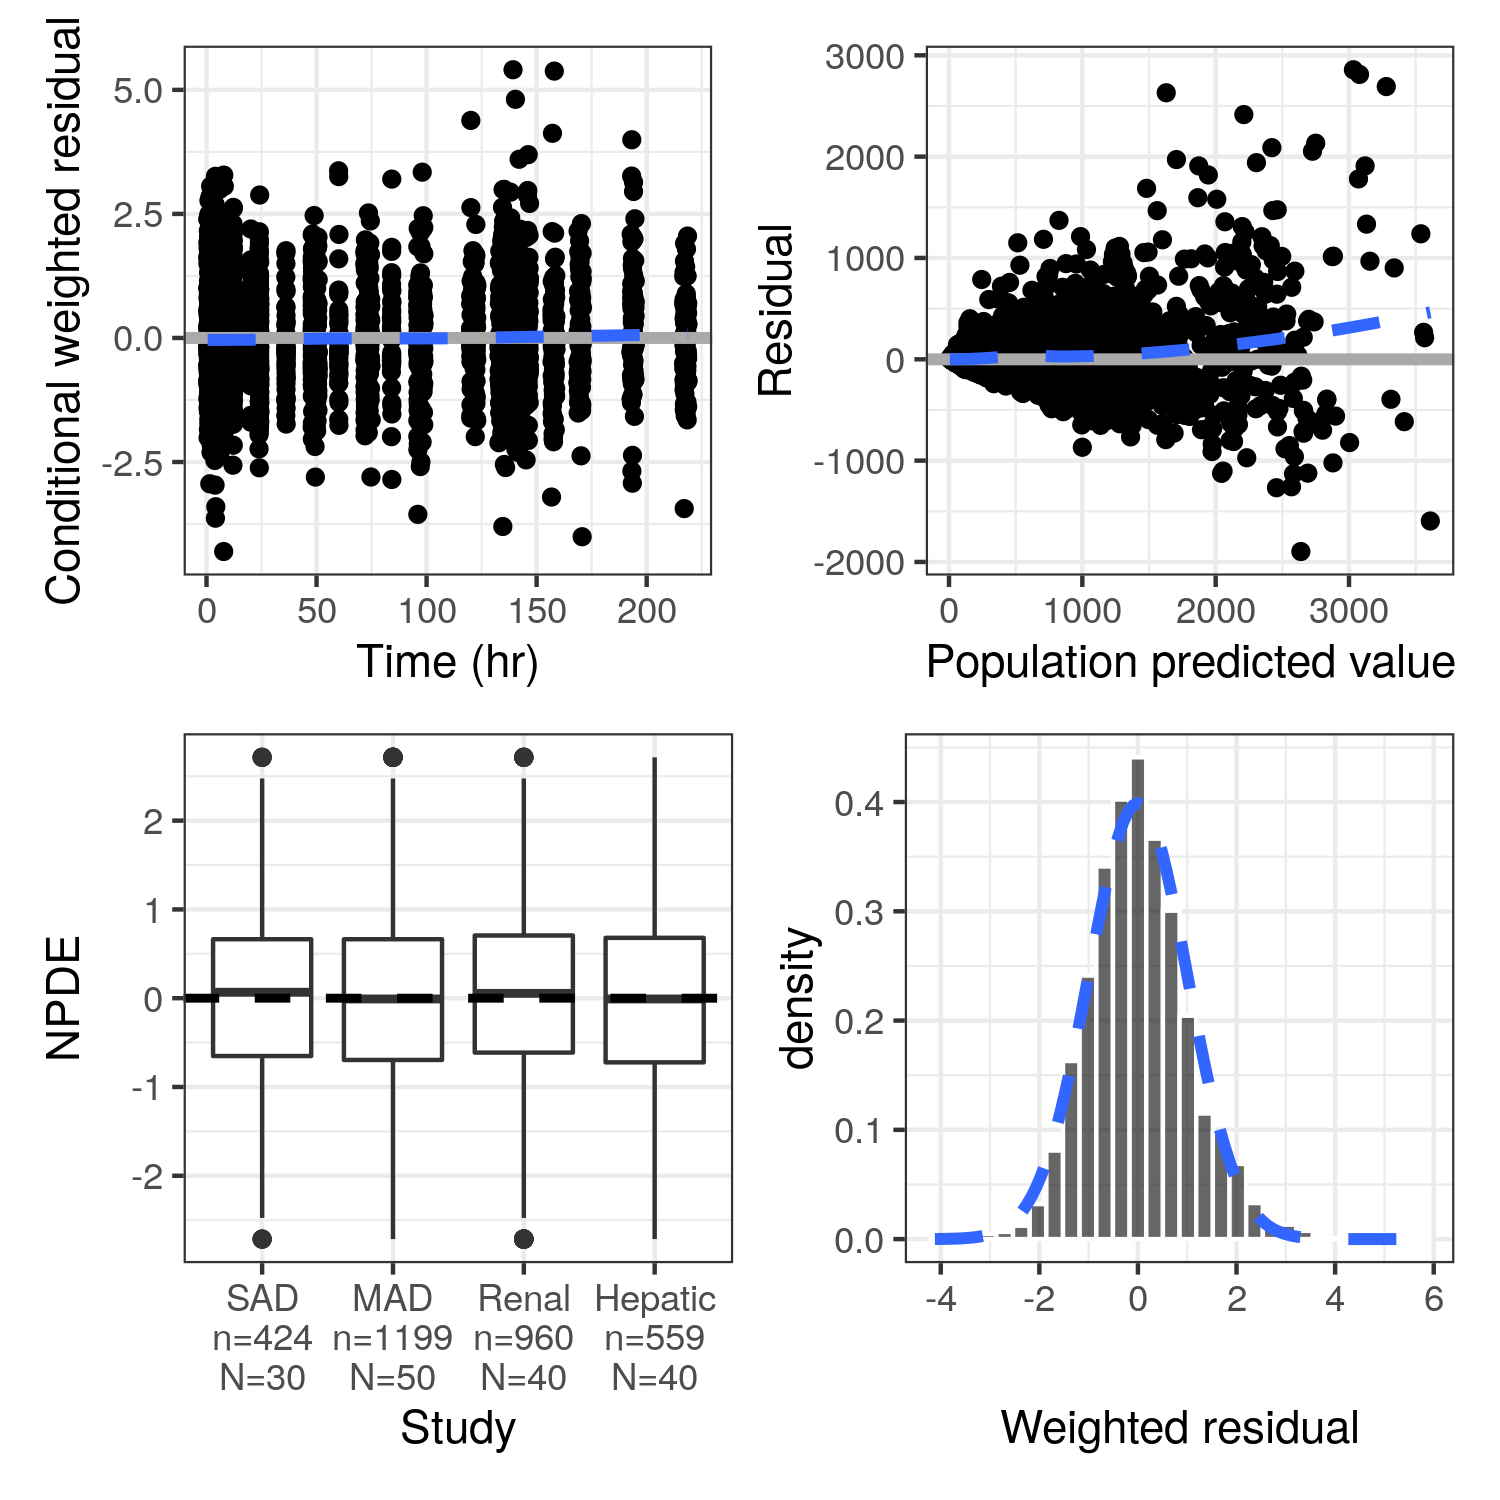
\includegraphics[scale=0.5]{"images/res.png"}
		\end{minipage}

		\vspace{-3mm}
	\end{demobx}	
\end{minipage} % no space if you need them side by side

\hspace{0.667\linewidth}
\begin{minipage}[c]{0.333\linewidth}
	\vspace{-21.45cm} %%%% TODO - fix box heights
	\begin{demobx}[]
		% %%%%%%%%%%%% pmtables %%%%%%%%%%%%%%%%%%%%%%%%%%%%%%%%%%%%%%%%%%%%%%%%%%%%%%%%%	
		
		\begin{wrapfigure}{l}{0.2\textwidth}
			\vspace{-0.45cm}
			
\includegraphics[scale=0.175]{"images/metrum_pmtables_git_logo.png"} 
		\end{wrapfigure}
		% Text chunk at the top of the box
		The \pkgText{pmtables R package} helps you create summary tables commonly used in pharmacometrics, such as data summaries and continuous or categorical covariate summaries. Further, it helps you turn any R table into a highly customized tex table suitable for reports generated with LaTeX or Markdown. 
		\vspace{0.4cm}

		%%% Table
		\begin{minipage}[c]{0.55\textwidth} %% Code
			\vspace{-8mm}
			\desc{Data summary table}\newline
			\vspace{-0.25cm}
			\code{tab <- data \%>\% \hspace{4.5cm} } \vspace{-0.15cm}
			\code{\hspace{0.05cm} filter(EVID==0) \%>\%  \hspace{3.8cm}} \vspace{-0.15cm}
			\code{\hspace{0.05cm} pt\_data\_inventory(by=c("Study"="STUDYc"))\%>\%} \vspace{-0.15cm}
			\code{\hspace{0.05cm} stable() \hspace{5.6cm}} \vspace{-0.15cm}
		\end{minipage}	
		\begin{minipage}[c]{0.4\textwidth} %% Figure
			\vspace{-0.5cm}
			% Summary table
			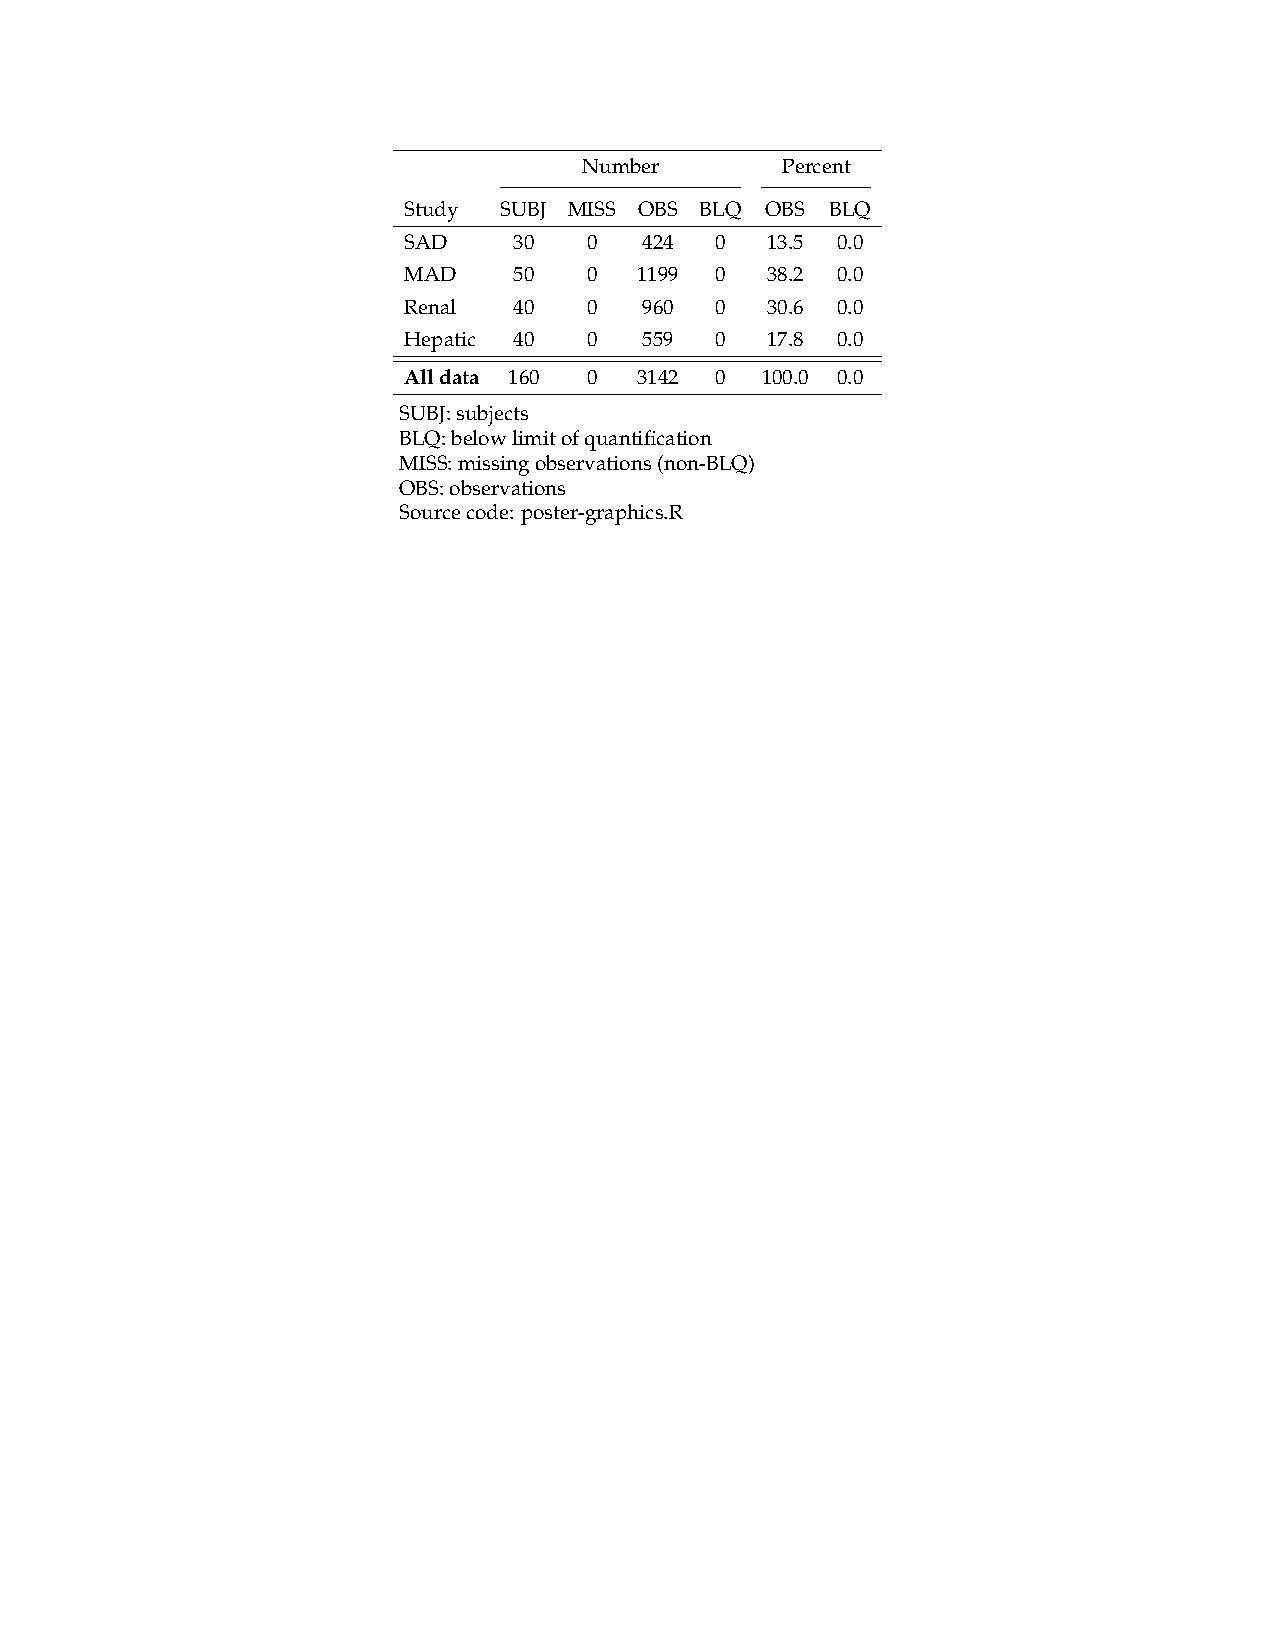
\includegraphics[scale=0.1]{"images/pk-data-sum.png"}
		\end{minipage}
		\vspace{-2mm}



% }
	\end{demobx}	
\end{minipage} % no space if you need them side by side



\hspace{0.667\linewidth}
\begin{minipage}[c]{0.333\linewidth}
	\vspace{-8cm} %%%% TODO - fix box heights
	\begin{demobx}[]
		% %%%%%%%%%%%% pmforest %%%%%%%%%%%%%%%%%%%%%%%%%%%%%%%%%%%%%%%%%%%%%%%%%%%%%%%%%	
		
		\begin{wrapfigure}{l}{0.2\textwidth}
			\vspace{-6mm}\hspace{-4mm}
			
\includegraphics[scale=0.0775]{"images/pmForest-Hex.png"} 
		\end{wrapfigure}
		% Text chunk at the top of the box
		The \pkgText{pmforest R package} helps you visualize the covariates of interest in your analysis by creating grouped displays of point estimates and variability ranges for any kind of continuous data. 
		
		% \vspace{-0.5mm}
		\hspace{-6mm}
		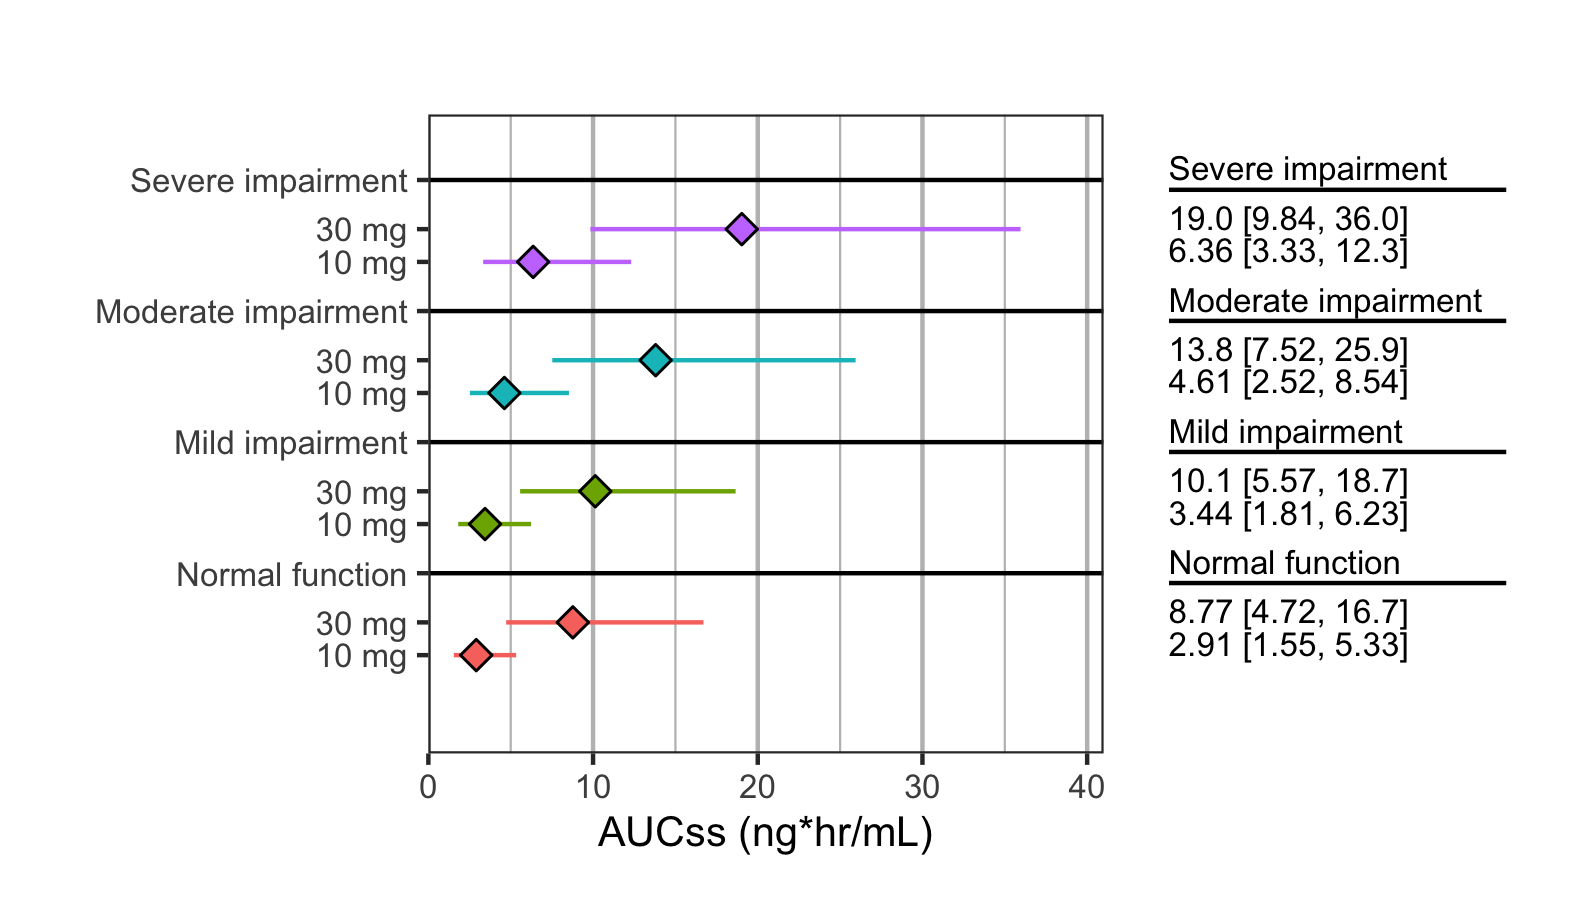
\includegraphics[scale=0.18]{"images/forest.png"}
		\vspace{-7mm}

	\end{demobx}	
\end{minipage} % no space if you need them side by side

\vspace{-3mm}

} %% Close - Large box around spot-lighted packages 


%%%%%%%% Other packages %%%%%%%%%%%%%%%%%%%%%%%%%%%%%%%%%%%%%%%%%%%%%%%%%%%%%%

\headerbox{Other Packages}{name=otherpkgs,column=0,below=pkgs}{
	\begin{itemize}
		\item The \pkgText{mrgsolve R package} allows you to simulate from ODE-based population PK/PD and QSP models. 
		% \vspace{-0.2cm}
		\item The \pkgText{mrggsave R package} can be used to save images in bulk and annotate figures with the file names of the source code and the output image. 
		% \vspace{-0.2cm}
		\item The \pkgText{lastdose R package}  can be used to calculate time after dose. 
		% \vspace{-0.2cm}
		\item The \pkgText{MPN (MetrumRG Package Network) and pkgr} tools allow you to create and manage curated, reproducible R package environments.

	\end{itemize}
}


%%%%%%%% Resources %%%%%%%%%%%%%%%%%%%%%%%%%%%%%%%%%%%%%%%%%%%%%%%%%%%%%%

\headerbox{Visit our Expo website}{name=resources,column=1,below=pkgs}{
	\vspace{-1.5mm}
	\begin{minipage}[c]{0.3\linewidth}
		
\includegraphics[scale=0.25]{"images/qrcode-merge.png"}
	\end{minipage}
	\begin{minipage}[c]{0.66\linewidth}
		% \Large{\greenBF{Visit our Expo website}}
		% \normalsize 

		You'll find:
		\vspace{-3mm}
		\begin{itemize}
			\item Our approach to project set-up, data assembly, modeling and simulation activities, and reporting.
			\vspace{-2mm}
			\item Access to example code in a Github repository.
			\vspace{-2mm}
			\item Information and vignettes on MetrumRG's suite of tools.
		\end{itemize}
	\end{minipage}
	\vspace{-1mm}
}

%%%%%%%% References %%%%%%%%%%%%%%%%%%%%%%%%%%%%%%%%%%%%%%%%%%%%%%%%%%%%%%

\headerbox{References}{name=references,column=2,below=pkgs}{
	 \begin{flushleft}
	 \bibliographystyle{custom}
\renewcommand\refname{}
	\vspace{-4mm}
	\bibliography{bib-acop-2022}
	\end{flushleft}
}
%%%%%%%%%%%%%%%%%%%%%%%%%%%%%%%%%%%%%%%%%%%%%%%%%%%%%%%%%%%%%%%%%%%%%%%%%%%%%%%%
%%%%%%%%%%%%%%%%%%%%%%%%%%%%%%%%%%%%%%%%%%%%%%%%%%%%%%%%%%%%%%%%%%%%%%%%%%%%%%%%

% %\headerbox{Acknowledgements}{name=acknowledgements,column=2,below=references, span=1}{
% %This work was funded by NameOfSponsorHere.
% %}
\headerbox{
	\small ~~Presented at the American Conference on Pharmacometrics; 30 October - 4 November 2022
	~~~~~~~~~~~~~~~~~~~~~~~~~~~~~~~~~~~~~~~~~~~~~~~~~~~~~~~~~~~~~~~~~~~~~~~~~~~~~~~~~~~~~~~~~~~~~~~	
Copies available at: www.metrumrg.com/all-publications 


~~~~~~~~~~~~~~~~~~~~~~~~~~~~~~~~~~~~~~~~~~~~~~~~~~~~~~~~~~~~~~~~~~~~\
\copyright\ Metrum Research Group 2022
}
{name=footer,column=0,span=3,below=references,textborder=none,headershape=rectangle,headerborder=none}{}

\end{poster}
\end{document}